\chapter{Physically Based Animation}
\section{Animation}
Given a particle in space, the animation of it refers to how its position in
space at the next time step is worked out. For the purposes of this thesis we
shall classify animation as either being \textit{kinematic} or \textit{dynamic}.
Classifying them as such does not imply there are only two
techniques of animation. Watt \cite{Watt} separates techniques for
animation into 5 different (rigid body animation, articulated structure
animation, dynamic simulation, particle animation and behavioural animation) but
not mutually exclusive categories. It simply suits this Thesis that a
distinction is made between kinematic and dynamic animation. 

Kinematic animation, as described by Watt \cite{Watt}, involves the
specification of motion without considering the force or energy applied to a
particle. Contemporary forms of animation used in games \cite{Eberly,
MollerHaines, Watt} and computer animated movies \cite{Watt} make heavy use of
this form of animation. A popular technique called \textit{key frame} animation
is often used to animate an object. In key frame animation a series of points in
space is specified and the particle moves to those points using some form of
interpolation. In general the key frames are generated by a human animator who
manually specifies key frames using a modelling package, or via motion capture
or using a \textit{procedural} animation. Procedural animation allows the key frames to be
generated using a function and is useful if the motion of an object can be
represented by a function. For example the walk cycle of character can have its
key frames generated using sinusoidal function. This relieves the animator from
having to manually generate positions and orientations.

Interpolation allows the gaps between the key frames defined to be filled.
Translations can be interpolated using linear interpolation, which results in
the particle moving along the straight line between any two points. This 
gives adequate results for a path consisting of 2 points however for a path
consisting of more that 2 translation key frames the movement of the particle
will be discontinuous. Continuity of level $C^1$ (see footnote\footnote{The
notation $C^n$ denotes the set of functions for which an $nth$ derivative
exists}) can be preserved by using Hermite interpolation \cite{MollerHaines}.
The interpolation of orientations is more difficult. An orientation can be
represented using Euler angles or quaternions. Interpolation of orientations
represented using Euler angles is problematic \cite{Watt}. Quaternions, on the
other hand, can be interpolated using spherical linear interpolation
\cite{Shoemake} such that the angular velocity will remain constant between 2
orientations. 

Note that the descriptions given above are essentially kinematic. That is, they
involve the specification of motion without considering forces or energy. As
soon as forces are considered the problem becomes known as dynamic simulation or
physically based animation \cite{Watt, Eberly}. The majority of physically based
animation uses Newtonian mechanics to produce the desired motion. The basic
process starts from specifying a force on a particle and solving Newton's 2nd
law $\mathbf{F} = m\ddot{\mathbf{x}}$ for $\mathbf{x}$. A motivation for using
dynamics in computer animation comes from the realization that some things are
beyond a human animators ability to realistically key frame. For example, the
motion of a double pendulum or the ragdoll effect that is popular in games would
be hard to hand animate. Cohen et al. \cite{Cohen} notes that dynamic simulation
provides the ability to automatically generate motion but removes the control
from the animator. An example that illustrates this problem is animating a
character falling down a flight of stairs. It is possible to physically animate
the process however what if the animator wants to have the character waving an
arm while tumbling? A solution for this is proposed by Laszlo et al. in
\cite{InteractiveControl}.

In this thesis only the dynamics of particles are examined. The 
dynamics of a rigid body with volume are more complicated. For example consider
applying a force to an object, like a cylinder. If the force is applied
through the center of mass then the object will not rotate. However, if the
force is applied off center, then a rotation and a translation will occur. This
rotational force is called the torque $\tau$. The torque on a rigid body is 
given by the following equation
\begin{equation}
	\label{Eqn:Torque}
	\mathbf{\tau} = \mathbf{r} \times \mathbf{F}
\end{equation}
where $\mathbf{r}$ is the position relative to the center of mass of the body
acted on by the force \cite{Otte}. Therefore, if the relative position is
$\mathbf{0}$ (i.e. the force is acting through the center of mass), then
$\mathbf{\tau} = \mathbf{0}$, which is what we expect. If the force is applied
off center the body will acquire a higher kinetic energy because it will
have an angular and kinetic velocity \cite{Watt}. To incorporate this requires
some way to specify how the mass is distributed about the body. This is done
using the moment of inertia, which is given by the following equations.
\[
I_x = \int (y^2 + z^2)dm
\]
\[
I_y = \int (x^2 + z^2)dm
\]
\[
I_z = \int (x^2 + y^2)dm
\]

If the body is not symmetric the products of inertia are also required.
\[
I_{xy} = \int xy dm
\]
\[
I_{xz} = \int xz dm
\]
\[
I_{yz} = \int yz dm
\]

These are placed into a 3x3 matrix known as the inertia tensor
\[
\mathbf{I} = 
\begin{bmatrix}
	I_x &\:& -I_{xy} &\:& -I_{xz} \\
	-I_{xy} &\:& I_{y} &\:& -I_{yz} \\
	-I_{xz} &\:& -I_{yz} &\:& I_{z}
\end{bmatrix}
\]
For more on rotational dynamics see \cite{Otte, Goldstein, Watt}.

\section{Collision Detection} 
\label{Sec:CollisionDetection} 
Collision detection and response is an important part of any physically based
animation system.  Collision detection can be separated into broad and narrow
phase algorithms.  Broad phase algorithms try to cull objects that cannot
possibly collide. Narrow phase algorithms try to determine the exact point of
collision.  These algorithms exploit spatial and temporal coherence. In other
words if an object is at a point, p, then at the next time step it is assumed
that its location will not be far from p. A naive broad phase algorithm has an
order of $O(n^2)$ and each object in the scene will be compared with every other
object in the scene. Probably the most popular way to do broad phase collision
detection is by using hierarchical bounding volumes. Bounding volumes also fit
nicely with a scene graph where the hierarchy is based on the spatial
relationship between the parent and child nodes (see the section on scene graphs
\ref{Sec:SceneGraph}).  The parent node's bounding volume encapsulates the
bounding volumes of the child nodes and if the parent's bounding volume does not
intersect an object of interest then the entire subgraph (i.e. the graph below
the parent node) can be ignored \cite{Eberly}. A problem with collision
detection is known as the time step weakness in which a relatively fast moving
object can pass through another object before the collision detection takes
place. Hubbard \cite{InteractiveColDet} shows that a moving object sweeps out a
parabolic horn shape in 4 dimensional space. To simplify the collision detection
the shape of the horn is approximated using a 4 dimensional trapezoid. An
intersection of these 4 dimensional trapezoids means that a collision 
occurs. This can eliminate the time step weakness problem.

Collision response is application dependent. In a proper dynamical simulation a
collision is modelled as large impulsive force acting over a short time frame
\cite{Watt, Otte}. An advanced simulation would model the friction between the
surfaces, energy loss and deformation of surfaces. 

Collision detection in this thesis is simple and limited to a narrow phase
algorithm. No broad phase analysis is done. The scenes rendered do not have
enough objects to warrant a broad phase analysis. Collisions between particles
and meshes are detected using a ray triangle intersection test. Collision
response amounts to a force being added in the direction of the plane normal of
the triangle the particle collides with. The magnitude of the force depends on
the penetration depth of the particle, which is calculated during the ray
triangle intersection test, and a user defined constant. This is a
penalty method where the constant determines the springiness of the collision.
An algorithm for the fast detection of penetration
depth is detailed by Kim et al. \cite{FastPenDepth}.

\section{Penalty Methods}
\label{Sec:PenaltyMethod}
A penalty method implements a constraint on a particle by imposing a force on a
particle when it breaks a condition. This force may not exist in real life. For
example consider simulating a ball hitting the floor. A penalty method will let
the ball pass through the ground and the create a reactionary force with a
magnitude proportional to the penetration depth and direction in the direction
of the surface normal of the ground. Physically this is incorrect since the ball
never passes through the ground. However the visual result, which is what we are
concerned with here since this is computer graphics, is realistic enough. One
way to implement a penalty method is by using a mass spring system.
\subsection{Generalized Mass Spring System}
\label{SubSec:MassSpring}
For a generalized mass spring system the goal is to work out the position of
each particle at a given time. Using Newtonian mechanics this means we need to
know the acceleration of each particle. The acceleration can be computed once we
know the force on a particle. The force on a particle is the sum of the forces
generated by the joining springs. Since we know how to compute the force
generated by a spring (the spring constant multiplied by its displacement from
resting length) we can compute the force on a particle. Hence the equation for
the magnitude of the force on a particle $i$ is
\begin{equation}
   \label{magforce}
	F_i = \sum_{j=0}^{n}k_j\left(\left|{x}_i -
      {x}_j\right|-l_j\right)        
\end{equation}
where $n$ is the number of connecting springs, $k_j$ is the spring constant and
$l_j$ is the rest length of the spring. In order to make this usable the
direction that the force is acting in needs to be considered. Representing the
position of the particle by the vector 
\[
    \mathbf{x} = \begin{bmatrix}
                    x\\
                    y\\
                    z
                 \end{bmatrix}
\] 
Then the direction vector between two particles is
\[
    \mathbf{r}_{ij} = \mathbf{x}_j - \mathbf{x}_i
\]
and the normalized direction vector is 
\[
    \frac{\mathbf{r}_{ij}}{\left|\mathbf{r}_{ij}\right|}
\]
Now that we have a direction in which to apply the magnitude of the force,
that won't alter the final magnitude, since it is normalized, an  
equation for the force on particle $i$ in vector notation is 
\begin{equation}
\label{Eqn:UndampedSpring}
    \mathbf{F}_i = \sum_{j=0}^{n}k_j\left(\left|\mathbf{r}_{ij}\right|-l_j\right)
                    \frac{\mathbf{r}_{ij}}{\left|\mathbf{r}_{ij}\right|}
\end{equation} 
When simulating systems on a computer inaccuracies accumulate as a result of the
the numerical methods used (see Appendix \ref{Cha:DESolvers}). This can
result in system instability where energy is added to the system. The energy of
a perfect system should remain constant. In reality most systems will lose
energy due to friction. For the mass spring system some damping terms are
introduced to give the final equation. A common way to
model damping is to add an opposing force that has a magnitude proportional to
the rate of change of some property. In the case of the movement of the particle
through the air the property is distance, hence equation \ref{Eqn:UndampedSpring}
becomes
\begin{equation}
    \label{Eqn:DampedSpring}
      \mathbf{F}_i =
      \sum_{j=0}^{n}\left(k_j\left(\left|\mathbf{r}_{ij}\right|-l_j\right) 
                    + k_d\frac{d}{dt}\left|\mathbf{r}_{ij}\right|\right)
                    \frac{\mathbf{r}_{ij}}{\left|\mathbf{r}_{ij}\right|} 
\end{equation}
where $k_d$ is the constant of damping that we are free to set to get the
desired behaviour.

The mass spring system is a versatile model for producing realistic looking
simulations. With a little imagination it can be applied to simulate a variety
of phenomenon like cloth and rigid links between between particles. It
also interacts well with other bodies that might be in the simulation.
Stiffness (see Appendix \ref{Cha:DESolvers}) is a problem to watch out for.

\section{Geometric Constraints} The goal in constraint based dynamics is to
create a force that can be applied to a particle. A constraint is a geometric
condition imposed on a particle \cite{BarzelBarr}. From the constraint a
resultant force is generated.  This constraint force is added to the other
forces acting on the particle and we can proceed with the simulation as usual.
Geometric constraints are described and categorized in \cite{Goldstein,
ComputationalDynamics, Lee}. The constraints encountered in this thesis are
holonomic constraints that have no explicit dependence on time. In other words
the constraint is of the form $\mathbf{C(q)} = \mathbf{0}$. A method for
animation using space-time constraints is detailed by Witkin et al. in
\cite{SpacetimeConstraints}. An example of a holonomic constraint is the
equation $\vert \mathbf{a} - \mathbf{b} \vert - d = 0$. It describes a test to
see if the distance between points $\mathbf{a}$ and $\mathbf{b}$ is equal to a
constant distance, $d$. A non-holonomic constraint is $\vert \mathbf{a} -
\mathbf{b} \vert - d < 0$ which specifies that the distance between the points
should always be less than $d$. It is postulated that it may be possible in some
restricted circumstances that a non-holonomic constraint in 2 dimensions can be
turned into a holonomic constraint in 3 dimensions. The reason for this can be
explained as follows. Imagine a 2D constraint of $\vert \mathbf{a} - \mathbf{b}
\vert - d = 0$. This can be used to constrain a particle to remain a fixed
distance from point $\mathbf{a}$ and in 2 dimensions the allowable positions
fall on the circle centered at $\mathbf{a}$ with a radius $d$. Changing to the
following non-holonomic constraint $\vert \mathbf{a} - \mathbf{b} \vert - d < 0$
means that positions inside the circle are now valid.  These positions are the
projections of the allowed positions given by the fixed distance holonomic
constraint in 3 dimensions, since the this 3 dimensional constraint traces out a
sphere. Further investigation of this idea was not within the scope of this
thesis.

\subsection{Pendulum or Bead on a Wire System}
\label{SubSec:Pendulum}
The following explanation is based on \cite{PBMNotes} and \cite{Otte}.  Consider
a bead constrained to move along a circular path. An external force (gravity for
example) is applied to the particle. We desire that there be a constraint force
that will compensate for the effects of gravity on the bead such that the bead
remains on the circular path. From this description we can say that the
constraint force must depend on the external forces (in this case gravity) and
the position of the particle. 

The constraint itself can be described as $C(\mathbf{x)}$ where $\mathbf{x}$ is
the position of the particle and $C(\mathbf{x)} = 0$ when the constraint is
satisfied. For the system in question, where the circle is centered at (0,0) the
constraint function is $C(\mathbf{x)} = \frac{1}{2}(\|\mathbf{x}\|^2 - d^2)$.
The $\frac{1}{2}$ is there to simplify the differentiation. This constraint describes 
the set of legal positions of the particle. Therefore the first derivative of
the constraint function with respect to time represents the legal velocity and is given by
\begin{equation}
    \label{Eqn:LegalVelocity}
    \dot{C(}\mathbf{x})=\mathbf{x}\cdot\dot{\mathbf{x}}
\end{equation}
The second derivative of the constraint function represents the legal
acceleration of the particle and is given by
\begin{equation}
    \label{Eqn:LegalAcceleration}
    \ddot{C(}\mathbf{x})=\ddot{\mathbf{x}}\cdot{\mathbf{x}} + 
    \dot{\mathbf{x}}\cdot\dot{\mathbf{x}}
\end{equation}
From Newtonian mechanics we know that
$\mathbf{f + \hat{f}} = m\mathbf{\ddot{x}}$ therefore
\[\mathbf{\ddot{x}} = \frac{\mathbf{f + \hat{f}}}{m}\] 
Substituting that into $\mathbf{\ddot{C}}$ gives
\begin{equation}
    \label{Eqn:ConstraintForce}
    \hat{\mathbf{f}}\cdot\mathbf{x} = 
    -\mathbf{f}\cdot\mathbf{x} - 
    m\dot{\mathbf{x}}\cdot\dot{\mathbf{x}}
\end{equation}
This gives a system of equations with two unknowns ($f.x$ and $f.y$). In order
to solve for them we need more information. This information is gleaned from the
observation that the constraint force should not add energy to the system.

The constraint force $\hat{\mathbf{f}}$ should not add energy to the system.
This is equivalent to saying that the constraint force must not do any work. For
a force to do work some component of it must be applied in the direction of
motion. If the constraint force is to do no work then any component of the force
must not be applied in the direction of motion. The direction of motion is given
by the legal velocities of the particle. A rule that describes the preceding ideas
regarding the the nature of the constraint force can be expressed mathematically
as $\hat{\mathbf{f}}\cdot\mathbf{\dot{x}}=0$ where
$\mathbf{\dot{x}}$ is a legal velocity of the particle. Since a legal velocity
satisfies the constraint \ref{Eqn:LegalVelocity} we can now say the following about
the nature of the constraint force
\begin{equation}
    \hat{\mathbf{f}}\cdot\dot{\mathbf{x}} = 0, \ \forall \ \dot{\mathbf{x}} \
    \vert \ \dot{\mathbf{x}}\cdot\mathbf{x}  = 0
\end{equation}
This statement says that the only valid constraint forces are orthogonal to the
velocity. It also says that the valid velocities are orthogonal to $\mathbf{x}$.
If all legitimate constraint forces must be orthogonal to the set of all valid
velocities, given by \ref{Eqn:LegalVelocity}, then it must be that the constraint
force is also in the collinear with $\mathbf{x}$.  
\begin{equation}
    \hat{\mathbf{f}}=\lambda\mathbf{x}
    \label{cforcesimple}
\end{equation} 
Substituting for $\mathbf{\hat{f}}$ in \ref{Eqn:ConstraintForce} gives
\begin{equation}    
    \lambda = \frac{-\mathbf{f}\cdot\mathbf{x} -
    m\mathbf{\dot{x}}\cdot\dot{\mathbf{x}}}{\mathbf{x}\cdot\mathbf{\dot{x}}}
    \label{Eqn:LambdaSimple}
\end{equation}
Once lambda is solved for it is a simple matter to compute the constraint force
$\mathbf{\hat{f}}$. Adding it to the force on the particle due to gravity gives
the total force.

\subsection{General Constraints}
\label{SubSec:GeneralConstraints}
The approach described here is based on the \cite{PBMNotes} and
\cite{Otte}. Ideally a system that allows for multiple particles governed by a
number of constraints is desirable. The system should allow us to specify the
constraints between rigid bodies and allow for the dynamic removal or addition
of bodies to the system. To do this we build on the ideas described in the
previous section and extend the system so that it caters for multiple particles
and arbitrary constraint functions. Each particle has a position vector
$\mathbf{x_1, x_2, x_3, ... }$. Assuming that the particles are in 3D then
define $\mathbf{q}$ such that it is a vector of those positions:
\[
    \mathbf{q} = 
    \begin{bmatrix}
        \mathbf{q}_{1}^T \: \mathbf{q}_{2}^T \: ... \: \mathbf{q}_{n}^T
    \end{bmatrix}^T
\]
Where
\[
    \mathbf{q}_i = 
    \begin{bmatrix}
        x\\
        y\\
        z\\
    \end{bmatrix}
\]
Each particle is acted on by a force. These forces are placed into a force vector
\[
    \mathbf{Q} =
    \begin{bmatrix}
        \mathbf{f}_1^T \: \mathbf{f}_2^T \: .... \: \mathbf{f}_n^T
    \end{bmatrix}
\]
where $\mathbf{f}_i$ represents the force on $\mathbf{q}_i$.


Define the mass matrix for the system to be a diagonal matrix whose diagonals
are the masses of the particles $\mathbf{M}=diag([m_1, m_1, m_1, m_2, m_2, m_2...m_n,
m_n, m_n])$. The size of the matrix is for particles in 3 dimensions is $3n*3n$
where $n$ is the number of particles in the system. The acceleration vector for
the system is given by    
\[
    \mathbf{\ddot{q}} = \mathbf{W}\left(\mathbf{Q} + \mathbf{\hat{Q}}\right) 
\]
where $\mathbf{W}$ is simply the inverse mass matrix and $\mathbf{\hat{Q}}$ is
the yet to be determined constraint force.

The next step is to define a more generic constraint function that can be used
to represent the legal positions, velocities and accelerations of the system of
particles. Starting from the positional constraint
\begin{equation}
    \label{constrpos}
    \mathbf{C}(\mathbf{q}) = \mathbf{0}
\end{equation}
we can derive a constraint for the legal velocities 
\[
    \mathbf{\dot{C}} = \frac{d\mathbf{C}}{dt} = \frac{\partial\mathbf{C}}{\partial\mathbf{q}}
        \frac{d\mathbf{q}}{dt}
\]
and a constraint to describe the legal accelerations
\[
    \mathbf{\ddot{C}} = \frac{d\mathbf{\dot{C}}}{dt} = \frac{d}{dt}\left(
        \frac{\partial\mathbf{C}}{\partial\mathbf{q}}\right)\mathbf{\dot{q}} +
        \frac{\partial\mathbf{C}}{\partial\mathbf{q}}\mathbf{\ddot{q}}
\]
The quantity $\frac{\partial\mathbf{C}}{\partial\mathbf{q}}$ represents the
derivative of a vector with respect a vector. This results in a matrix where
each element is the element by element derivative of $\mathbf{C}$ with respect
to $\mathbf{q}$. This matrix is called the Jacobian of $\mathbf{C}$
\begin{equation}
    \label{Eqn:Jacobian1}
    \mathbf{J}=
    \begin{bmatrix}
        \mathbf{J}_1\\
        \mathbf{J}_2\\
        ...\\
        \mathbf{J}_i\\
        ...\\
        \mathbf{J}_n
    \end{bmatrix}
\end{equation}
And 
\begin{equation}
    \label{Eqn:Jacobian2}
    \mathbf{J}_i = 
    \frac{\partial \mathbf{C}_i}{\partial \mathbf{q}} = 
    \begin{bmatrix}
        \frac{\partial C_{i1}}{\partial q_0} \frac{\partial C_{i1}}{\partial
        q_1} ... \frac{\partial C_{i1}}{\partial q_n}\\
        ...\\    
        \frac{\partial C_{im}}{\partial q_0} \frac{\partial C_{im}}{\partial
        q_1} ... \frac{\partial C_{im}}{\partial q_n}\\
    \end{bmatrix}
\end{equation}
It is important to note that the number of rows in $\mathbf{J}_i$ is contingent
upon the number of rows in $\mathbf{C}_i$. As we shall see later $\mathbf{C}_i$
is a constraint function that can be a scalar or a vector.
\ref{Eqn:Jacobian1} lets rewrite the above equations more concisely a
\begin{equation}
    \label{constrvel}
    \mathbf{\dot{C}} =
    \mathbf{J}\mathbf{\dot{q}} =
    \mathbf{0}
\end{equation}
and
\begin{equation}
    \label{constracc}
    \mathbf{\ddot{C}} =
    \mathbf{\dot{J}}\mathbf{\dot{q}} + \mathbf{J}\mathbf{\ddot{q}} =
    \mathbf{0}
\end{equation}
Since $\mathbf{\ddot{q}} = \mathbf{W}\left(\mathbf{Q} + \mathbf{\hat{Q}}\right)$
substituting for $\mathbf{\ddot{q}}$ in \ref{constracc}
\begin{equation}
    \mathbf{\dot{J}}\mathbf{\dot{q}} + 
    \mathbf{J}\mathbf{W}\left(\mathbf{Q} + 
    \mathbf{\hat{Q}}\right) =
    \mathbf{0}
\end{equation} 
\begin{equation}
    \label{Eqn:GeneralConstraintForce}
    \mathbf{JW\hat{Q}} = 
    -\mathbf{\dot{J}\dot{q}} -  
    \mathbf{JWQ} =
    \mathbf{0}
\end{equation}
This is a similar equation to \ref{Eqn:ConstraintForce}. In
\ref{Eqn:GeneralConstraintForce} the unknown quantity is $\mathbf{\hat{Q}}$. 
As in the bead on the wire example, the constraint force $\mathbf{\hat{Q}}$ must
not contribute any energy to the system. Therefore the constraint force must act
orthogonally to the direction of motion. Since the direction of motion is given
by the velocity of the particle, the following condition must be met
\[
    \mathbf{\hat{Q}\cdot\dot{q}} = 0 
\]
where the velocities, $\mathbf{\dot{q}}$, satisfy \ref{constrvel}. 
\[
    \mathbf{\hat{Q}\cdot\dot{q}} = 0, \ \forall 
    \mathbf{\dot{q}} \ \vert \ \mathbf{J\dot{q}} = \mathbf{0}  
\]
The statement that $\mathbf{J\dot{q}} = \mathbf{0}$ means that each row of
$\mathbf{J}$ is orthogonal to $\mathbf{q}$. In other words $\mathbf{J}_i^T \cdot
\mathbf{\dot{q}} = 0$ where $\mathbf{J}_i$ is row $i$ of matrix $\mathbf{J}$.
Combine this with the fact that $\mathbf{\hat{Q}\cdot\dot{q}} = 0$ means that
all rows of $\mathbf{J}$ point in the same direction as $\mathbf{\hat{Q}}$.
Hence $\mathbf{J}_i$ is a scalar multiple of $\mathbf{\hat{Q}}$. This means that
we can write $\mathbf{\hat{Q}}$ as a linear combination of the rows of
$\mathbf{J}$
\begin{equation}
	\label{Eqn:ConForce}
    \mathbf{\hat{Q}} = \mathbf{J}^T\mathbf{\lambda}
\end{equation}
Substituting this into equation \ref{Eqn:GeneralConstraintForce} gives
\begin{equation}
    \label{Eqn:LambdaGeneral}
    \mathbf{JWJ}^T \mathbf{\lambda} = 
    -\mathbf{\dot{J}\dot{q}} -  
    \mathbf{JWQ} =
    \mathbf{0}
\end{equation}
Assuming that we are given enough information about the constraint function we
can compute $\mathbf{J}$ and $\mathbf{\dot{J}}$ and then solve this equation for
$\mathbf{\lambda}$ and as a result solve for $\mathbf{\hat{Q}}$.

Most of the following constraints are derived in \cite{Otte}. However the method
presented here is marginally different. We use the proof in
Appendix \ref{Cha:SimpleProof} as opposed to the vector matrix dot product used in
\cite{Otte}

\subsection{Fixed Distance Constraint}
\label{SubSec:FDConst}
A fixed distance constraint is used to enforce a rigid link between two bodies in
the system. The particles positions in the system are denoted by
\[
    \mathbf{q} = 
    \begin{bmatrix}
        \mathbf{q}_1\\
        \mathbf{q}_2\\
        ...\\        
        \mathbf{q}_n
    \end{bmatrix}
\] 
And the constraint vector contains the constraints pertaining to the system.
\[
    \mathbf{C} =
    \begin{bmatrix}
        \mathbf{C}_1\\
        \mathbf{C}_2\\
        ...\\        
        \mathbf{C}_n\\
    \end{bmatrix}
\]
Let one of these constraints, $C_k$, be a fixed distance constraint. Obviously
the constraint for $C_k$ must be specified in terms of the particles positions
in the system, therefore the general form of the fixed distance constraint is 
\begin{equation}
    \label{Eqn:LegalPosPlain}
    C_k = \vert\mathbf{q}_i - \mathbf{q}_j\vert - d = 0
\end{equation}
Since we will need to know the legal velocities, we will need to take to the
derivative of \ref{Eqn:LegalPosPlain}. An equivalent way to describe a fixed
distance constraint is 
\begin{equation}
    \label{Eqn:LegalPos}
    C_k = \frac{1}{2}\left(\mathbf{q}_i - \mathbf{q}_j\right)\cdot\left(\mathbf{q}_i -
    \mathbf{q}_j\right) - d^2 = 0
\end{equation}
This simplifies the differentiation.
In order to solve for \ref{Eqn:LambdaGeneral} we need to evaluate $\mathbf{J}$ and
$\mathbf{\dot{J}}$.
From \ref{Eqn:Jacobian2} we know that
\begin{equation}
    \label{Eqn:JacobianFixedDist1}
    \mathbf{J}_k = \frac{\partial C_k}{\partial \mathbf{q}} =
    \frac{\partial C_k}
    {\partial
        \begin{bmatrix}
            \mathbf{q}_1 \:
            \mathbf{q}_2 \:
            \cdots \:
            \mathbf{q}_i \:
            \cdots \:
            \mathbf{q}_j \:
            \cdots \:
            \mathbf{q}_m
        \end{bmatrix}^T
    }
\end{equation}
Because $C_k$ is in terms of only $\mathbf{q}_i$ and $\mathbf{q}_j$,
\ref{Eqn:JacobianFixedDist1} simplifies to
\begin{equation}
    \label{Eqn:JacobianFixedDist2}
    \mathbf{J}_k = 
    \begin{bmatrix}
    \mathbf{0}^T\:
    \mathbf{0}^T\:
    ...\:
    \displaystyle\frac{\partial C_k}{\partial \mathbf{q}_i}\:
    ...\:
    \displaystyle\frac{\partial C_k}{\partial \mathbf{q}_j}\:
    ...\:
    \mathbf{0}^T
    \end{bmatrix}
\end{equation}  
All that's left to do is solve for $\displaystyle\frac{\partial C_k}{\partial \mathbf{q}_i}$ and
$\displaystyle\frac{\partial C_k}{\partial \mathbf{q}_j}$. 
Using \ref{ApdxB:Proof1}
\begin{equation}	
    \frac{\partial{C_k}}{\partial\mathbf{q}_i} = \\
    (\mathbf{q}_i-\mathbf{q}_j)^T
    \begin{bmatrix}
    \displaystyle\frac{\partial (q_{i1}-q_{j1})}{\partial q_{i1}} \: \displaystyle\frac{\partial (q_{i2}-q_{j2})}{\partial q_{i1}} \: \displaystyle\frac{\partial (q_{i3}-q_{j3})}{\partial q_{i1}}\\
    \displaystyle\frac{\partial (q_{i1}-q_{j1})}{\partial q_{i2}} \: \displaystyle\frac{\partial (q_{i2}-q_{j2})}{\partial q_{i2}} \: \displaystyle\frac{\partial (q_{i3}-q_{j3})}{\partial q_{i2}}\\
    \displaystyle\frac{\partial (q_{i1}-q_{j1})}{\partial q_{i3}} \: \displaystyle\frac{\partial (q_{i2}-q_{j2})}{\partial q_{i3}} \: \displaystyle\frac{\partial (q_{i3}-q_{j3})}{\partial q_{i3}}\\
    \end{bmatrix} = \\
    (\mathbf{q}_i - \mathbf{q}_j)^T \mathbf{I} = \\
    (\mathbf{q}_i - \mathbf{q}_j)^T
\end{equation}
Similarly
\begin{equation}
    \frac{\partial{C_k}}{\partial\mathbf{q}_j} = \\
    (\mathbf{q}_i-\mathbf{q}_j)^T
    \begin{bmatrix}
    \displaystyle\frac{\partial (q_{i1}-q_{j1})}{\partial q_{j1}} \: \displaystyle\frac{\partial (q_{i2}-q_{j2})}{\partial q_{j1}} \: \displaystyle\frac{\partial (a_3-q_{j3})}{\partial q_{j1}}\\
    \displaystyle\frac{\partial (q_{i1}-q_{j1})}{\partial q_{j2}} \: \displaystyle\frac{\partial (q_{i2}-q_{j2})}{\partial q_{j2}} \: \displaystyle\frac{\partial (a_3-q_{j3})}{\partial q_{j2}}\\
    \displaystyle\frac{\partial (q_{i1}-q_{j1})}{\partial q_{j3}} \: \displaystyle\frac{\partial (q_{i2}-q_{j2})}{\partial q_{j3}} \: \displaystyle\frac{\partial (a_3-q_{j3})}{\partial q_{j3}}\\
    \end{bmatrix} = \\
    (\mathbf{q}_i - \mathbf{q}_j)^T (-\mathbf{I}) = \\
    (\mathbf{q}_j - \mathbf{q}_i)^T
\end{equation}
Therefore the Jacobian for a fixed distance constraint is a row matrix
\begin{equation}
    \label{Eqn:FixedDistConstraintJacobian}
    \mathbf{J}_k = 
    \begin{bmatrix}
        \mathbf{0}^T \: \mathbf{0}^T \: ... \left(\mathbf{q}_i -
        \mathbf{q}_j\right)^T 
        ... \left(\mathbf{q}_j - \mathbf{q}_i\right)^T ... \mathbf{0}^T 
    \end{bmatrix}
\end{equation}
This gives a formulation for the Jacobian of a fixed distance constraint that
is easy to implement in a program since it is given in terms of the particles'
positions. In a system with $\mathbf{J}_i$ forms part of the greater global
Jacobian matrix \ref{Eqn:Jacobian1}.

The time derivative of \ref{Eqn:FixedDistConstraintJacobian} is 
\begin{equation}    
    \dot{\mathbf{J}}_i =    
    \begin{bmatrix}
        \mathbf{0}^T \: \mathbf{0}^T \: ... \: \left(\dot{\mathbf{q}}_i -
        \dot{\mathbf{q}}_j\right)^T \: 
        ... \: \left(\dot{\mathbf{q}}_j - \dot{\mathbf{q}}_i\right)^T \: ... \:
        \mathbf{0}^T 
    \end{bmatrix}   
\end{equation}

With the information presented so far it is possible to implement a constrained
particle system using a series of fixed distance constraints.

\subsection{Fixed Position Constraint}
\label{SubSec:FixedPostionConstraint}
A fixed position constraint simple stops a particle from moving from a point
$\mathbf{p}$. The constraint
equation is given by
\begin{eqnarray}
	\label{Eqn:FixedPositionConstraint}
	\mathbf{C}_k = \mathbf{q}_i - \mathbf{p} = \mathbf{0} 
\end{eqnarray}
The legal velocities are given by
\begin{eqnarray}
	\label{Eqn:FixedPositionConVel}
	\mathbf{C}_k = \dot{\mathbf{q}}_i = \mathbf{0} 
\end{eqnarray}
which is intuitively what one would expect from a constraint that maintains a
fixed position.  In this case the only non-zero term of
\ref{Eqn:JacobianFixedDist1} is 
$\frac{\partial \mathbf{C}_k}{\partial \mathbf{q}_i}$.
\begin{equation}
	\label{Eqn:FixedPostionConstraint1}
	\frac{\partial \mathbf{C}_k}{\partial \mathbf{q}_i} = \frac{\partial
	\left[\mathbf{q}_i - \mathbf{p}\right]}{\partial \mathbf{q}_i} =
	\mathbf{I}
\end{equation}
Therefore \ref{Eqn:Jacobian2} for a fixed position constraint is
\begin{eqnarray}
	\label{Eqn:JacobianFixedPositionConstraint}
	\mathbf{J}_k = 
	\begin{bmatrix}
		\mathbf{0} \: \mathbf{0} \: \cdots \: \mathbf{I} \: \cdots \: \mathbf{0}
	\end{bmatrix}
\end{eqnarray}
The derivative of the Jacobian is simply a zero matrix. Note that these matrices
are not single row matrices, like those of the fixed distance constraint.

\subsection{Fixed Vector Constraint}
\label{SubSec:FixedVectorConstraint}
This constraint maintains the vector between to positions. It is a vector
constraint. 
\begin{eqnarray}
	\label{Eqn:FixedVectorConstraint}
	\mathbf{C}_k = (\mathbf{q}_j - \mathbf{q}_i) - \mathbf{v} = \mathbf{0} 
\end{eqnarray}
The legal velocities are then subject to the following constraint 
\begin{eqnarray}
	\label{Eqn:FixedVectorConVel}
	\dot{\mathbf{C}}_k = \dot{\mathbf{q}}_j - \dot{\mathbf{q}}_i = \mathbf{0} 
\end{eqnarray}
Again this makes sense and says that the relative velocities of the two
particles must be $\mathbf{0}$.
\begin{equation}
	\label{Eqn:FixedVectorConstraint1}
	\frac{\partial \mathbf{C}_k}{\partial \mathbf{q}_i} = -\mathbf{I}
\end{equation}
and
\begin{equation}
	\label{Eqn:FixedVectorConstraint2}
	\frac{\partial \mathbf{C}_k}{\partial \mathbf{q}_j} = \mathbf{I}
\end{equation}
Therefore \ref{Eqn:Jacobian2} for a fixed vector constraint is
\begin{eqnarray}
	\label{Eqn:JacobianFixedVectorConstraint}
	\mathbf{J}_k = 
	\begin{bmatrix}
		\mathbf{0} \: \cdots \: -\mathbf{I} \: \cdots \: \mathbf{I} \: \cdots \: \mathbf{0}
	\end{bmatrix}
\end{eqnarray}

$\dot{\mathbf{J}}$ is a zero matrix.

\subsection{Fixed Plane Constraint}
\label{SubSec:FixedPlaneConstraint}
A fixed plane constraint allows a particle to move within a plane only. Hence
the particle must at all times lie in the plane. A constraint for this is given
by the plane equation.
\begin{eqnarray}
	\label{Eqn:FixedPlaneConstraint}
	C_k = \mathbf{n}\cdot\mathbf{q}_i - d = 0
\end{eqnarray}
Then the Jacobian, given by \ref{Eqn:Jacobian2} is
\begin{eqnarray}
	\label{Eqn:JacobianFixedPlaneConstraint}
    \begin{split}
	\mathbf{J}_k & = \frac{\partial C_k}{\partial \mathbf{q}} \\ 
    & =  
	\begin{bmatrix}
		\mathbf{0}^T \: \mathbf{0}^T \: \cdots \: \frac{\partial
		C_k}{\partial \mathbf{q}_i} \: \cdots \: \mathbf{0}^T
	\end{bmatrix} \\
    & = 
	\begin{bmatrix}
		\mathbf{0}^T \: \mathbf{0}^T \: \cdots \:
		\mathbf{n}^T \: \cdots \: \mathbf{0}^T
	\end{bmatrix}
    \end{split}
\end{eqnarray}
And the derivative of the Jacobian is
\begin{eqnarray}
	\label{Eqn:DJacobianFixedPlaneConstraint}
	\dot{\mathbf{J}}_k = 
	\begin{bmatrix}
		\mathbf{0}^T \: \mathbf{0}^T \: \cdots \:
		\mathbf{0}^T \: \cdots \: \mathbf{0}^T	
	\end{bmatrix}
\end{eqnarray}

\subsection{Fixed Angle Constraint}
\label{SubSec:FixedAngleConstraint}
A fixed angle constraint maintains the angle between two vectors (inspired by
\cite{ODEFixedAngle}). A constraint for it is given by the following equation
\begin{eqnarray}
	\label{Eqn:FixedAngleConstraint}
	C_k = (\mathbf{q}_i - \mathbf{q}_j)\cdot(\mathbf{q}_k - \mathbf{q}_j) - \theta = 0
\end{eqnarray}
that says that the angle between the two vectors must equal $\theta$.
The legal velocity is given by
\begin{eqnarray}
	\label{Eqn:FixedAngleConstraintVel}
	\dot{C}_k = (\dot{\mathbf{q}}_i - \dot{\mathbf{q}}_j) \cdot 
                (\mathbf{q}_k - \mathbf{q}_j) +
                (\mathbf{q}_i - \mathbf{q}_j) \cdot
                (\dot{\mathbf{q}}_k - \dot{\mathbf{q}}_j) =
                0
\end{eqnarray}
The Jacobian is
\begin{eqnarray}
	\label{Eqn:JacobianFixedAngleConstraint}    
    \begin{split}
	\mathbf{J}_k & = \frac{\partial C_k}{\partial \mathbf{q}} \\ 
    & = 
	\begin{bmatrix}
		\mathbf{0}^T \: \mathbf{0}^T \: \cdots \: \frac{\partial
		C_k}{\partial \mathbf{q}_i} \: \cdots \frac{\partial
		C_k}{\partial \mathbf{q}_j} \: \cdots \frac{\partial
		C_k}{\partial \mathbf{q}_k} \: \cdots \mathbf{0}^T \\    
	\end{bmatrix}
    \end{split}
\end{eqnarray}
Working out the derivatives of $C_k$ with respect to $\mathbf{q}_i$, $\mathbf{q}_j$ and
$\mathbf{q}_k$ results in the following equations
\begin{eqnarray}
    \begin{split}
    \frac{\partial C_k}{\partial \mathbf{q}_i} & = (\mathbf{q}_i -
    \mathbf{q}_j)^T
    \frac{\partial [\mathbf{q}_k - \mathbf{q}_j]}{\partial \mathbf{q}_i} +
    (\mathbf{q}_k - \mathbf{q}_j)^T
    \frac{\partial [\mathbf{q}_i - \mathbf{q}_j]}{\partial \mathbf{q}_i} \\
    & =
    (\mathbf{q}_i - \mathbf{q}_j)^T \mathbf{0} + (\mathbf{q}_k - \mathbf{q}_j)^T \mathbf{1} \\
    & = 
    (\mathbf{q}_k - \mathbf{q}_j)^T
    \end{split}
\end{eqnarray}

\begin{eqnarray}
    \begin{split}
    \frac{\partial C_k}{\partial \mathbf{q}_j} & = (\mathbf{q}_i -
    \mathbf{q}_j)^T
    \frac{\partial [\mathbf{q}_k - \mathbf{q}_j]}{\partial \mathbf{q}_j} +
    (\mathbf{q}_k - \mathbf{q}_j)^T
    \frac{\partial [\mathbf{q}_i - \mathbf{q}_j]}{\partial \mathbf{q}_j} \\
    & =
    (\mathbf{q}_i - \mathbf{q}_j)^T (\mathbf{-1}) + (\mathbf{q}_k - \mathbf{q}_j)^T (\mathbf{-1}) \\
    & = 
    -(\mathbf{q}_i - \mathbf{q}_j)^T - (\mathbf{q}_k - \mathbf{q}_j)^T
    \end{split}
\end{eqnarray}

\begin{eqnarray}
    \begin{split}
    \frac{\partial C_k}{\partial \mathbf{q}_k} & = (\mathbf{q}_i -
    \mathbf{q}_j)^T
    \frac{\partial [\mathbf{q}_k - \mathbf{q}_j]}{\partial \mathbf{q}_k} +
    (\mathbf{q}_k - \mathbf{q}_j)^T
    \frac{\partial [\mathbf{q}_i - \mathbf{q}_j]}{\partial \mathbf{q}_k} \\
    & =
    (\mathbf{q}_i - \mathbf{q}_j)^T \mathbf{1} + (\mathbf{q}_k - \mathbf{q}_j)^T \mathbf{0} \\
    & = 
    (\mathbf{q}_i - \mathbf{q}_j)^T
    \end{split}
\end{eqnarray}
The time derivative of the Jacobian is then
\begin{eqnarray}
	\label{Eqn:DJacobianFixedAngleConstraint}
	\begin{split}
	\dot{\mathbf{J}}_k & = \frac{d}{dt}[\frac{\partial C_k}{\partial \mathbf{q}}] \\ 
    & = 
	\begin{bmatrix}
		\mathbf{0}^T \: \cdots \: \frac{d}{dt}[\frac{\partial
		C_k}{\partial \mathbf{q}_i}] \: \cdots \frac{d}{dt}[\frac{\partial
		C_k}{\partial \mathbf{q}_j}] \: \cdots \frac{d}{dt}[\frac{\partial
		C_k}{\partial \mathbf{q}_k}] \: \cdots \mathbf{0}^T     
	\end{bmatrix} \\
    & =
    \begin{bmatrix}
        \mathbf{0}^T \: \cdots (\dot{\mathbf{q}}_k - \dot{\mathbf{q}}_j)^T \: \cdots \:
        -(\dot{\mathbf{q}}_i - \dot{\mathbf{q}}_j)^T - (\dot{\mathbf{q}}_k - \dot{\mathbf{q}}_j)^T \:
        \cdots \: (\dot{\mathbf{q}}_i - \dot{\mathbf{q}}_j)^T \: \cdots \: \mathbf{0}^T
    \end{bmatrix}
    \end{split}
\end{eqnarray}

\subsection{Numerical Drift}
Over time the accuracy of the constraint force will deteriorate. The reason for
this is because the constraint, $\mathbf{C}_k$, that depends on the positions of
the particles. Since the positions of the particles are solved for using a
numerical differential equation solver, this introduces errors. The value of the
constraints that describe the legal positions, velocities and accelerations
depend on the positions, velocities and accelerations of the particles (see
\ref{constrpos}, \ref{constrvel}, \ref{constracc}). These will drift
from the original constraint and therefore incorrectly influence the final
constraint force.   

To compensate for numerical drift Witkin and Baraff describe a feedback term
that is based on Baumgarte stabilization \cite{Baumgarte}. A concise explanation
of the idea behind the technique can be found in \cite{ClinePai}. Instead of
solving for \ref{constracc}, solve for
\[
    \mathbf{\ddot{C}} = -k_s\mathbf{C} - k_d\mathbf{\dot{C}}
\]
where $k_s$ and $k_d$. This means that when the constraint velocities and
positions are 0 (i.e. the constraints are satisfied) the constraint acceleration
is also 0 and there is no error. If the constraint velocity or position is not
satisfied then a constraint correction force is added proportional to the error
in the velocity and position constraints. The final equation is then
\begin{equation}
\label{Eqn:LambdaStable}
\mathbf{JWJ}^T \mathbf{\lambda} = 
    -\mathbf{\dot{J}\dot{q}} -  
    \mathbf{JWQ} -k_s\mathbf{C} - k_d\mathbf{\dot{C}} = 0
\end{equation}

Note that in a recent publication \cite{PracticalDynamics}, it is advocated that
numerical integrator be a verlet integrator. One of its nice properties is that
it preserves the numerical flow of the system, which means that the system won't
suffer from numerical drift. This is not achievable using Euler or RK4
algorithms. 

\section{Lagrangian Dynamics}
\label{Sec:LagrangianDynamics}
So far dynamic simulation has been discussed in terms of Newtonian mechanics.
Some time was spent during this thesis learning about Lagrangian dynamics.
Mathematically, Lagrangian dynamics is categorized under variational calculus.
This field is concerned with finding the function, $y(x)$, that will
minimize or maximize (extremize) another function, $F$. More specifically we
want to find the function $y(x)$, that will minimize the following integral
\[
J = \int f(y(x), \dot{y}(x), x) dx
\]
It has been proved (see Goldstein \cite[pg 37 - 39]{Goldstein}) that a necessary condition for a
function, $y(x)$, to extremize the above integral is given by the following
equation, known as the Euler-Lagrange equation.
\begin{equation}
	\label{Eqn:EulerLagrange}
	\frac{\partial F}{\partial y} - \frac{d}{dx}\left(\frac{\partial F}{\partial \dot{y}}\right) = 0
\end{equation}
In a sense, variational calculus is a generalization of calculus itself since in
ordinary calculus one of the problems is to find a value for x that will
extremize $y(x)$. University level math courses often include a section on
variational calculus. It is probably
best to explain how to use this equation to derive the equations of motion by an
example that compares Newtonian and Lagrangian techniques.
\subsection{Deriving the Equations of Motion}
\label{Sec:DerivingTheEquationsOfMotion}
\subsubsection{Newtonian Technique}
\label{Sec:NewtonianTechnique}
Equations of motion for a single particle mass connected by two springs. The
springs connect the mass to two fixed points. We know the following.
\begin{figure}    
    \centering
	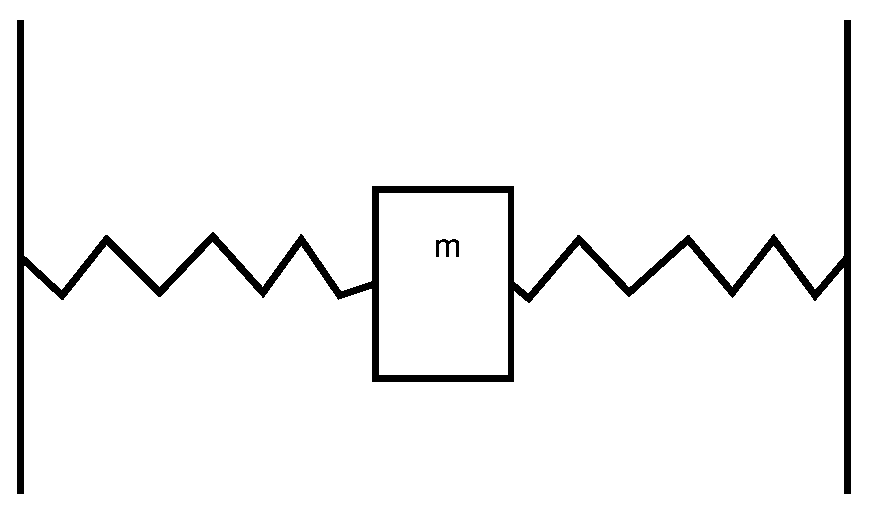
\includegraphics[width=0.5\textwidth]{SpringMassSystem}    
    \caption{\label{Fig:SpringMassSystem}A mass connected to 2 springs.}
\end{figure}
\begin{itemize}
\item $k_{0}$ = the spring constant of spring 0.
\item $k_{1}$ = the spring constant of spring 1.
\item $m$ = the mass of the particle.
\item $x(0) = x_0$ = the position of the particle at the starting time.
\item $\dot{x}(0) = 0$ = the velocity of the particle at the starting time.
\end{itemize}
The last two items are known as the initial conditions of the system since they
describe the state of the system at a starting time. With the information above
a solution to the following
\begin{itemize}
\item $x(t)$ = the displacement of the particle from its resting position.
\end{itemize}
can be derived using Newtonian methods.
Let $F_{0}$ be the force on the particle due to spring 0.
\begin{equation}
	F_{0} = -k_{0}x
\end{equation}
Let $F_{1}$ be the force on the particle due to spring 1.
\begin{equation}
	F_{1} = -k_{1}x
\end{equation}
Then the total force on the particle is
\begin{equation}
	F = F_{0} + F_{1}
\end{equation}
and using Newton's law $F = ma$
\[F = (-k_{0} - k_{1})x = m\ddot{x}	\]
\[\ddot{x} + \frac{(k_{0} + k_{1})}{m}x = 0\]
Letting $K = \frac{(k_{0} + k_{1})}{m}$
\begin{equation}
	\label{eqn_motion}
	\ddot{x} + Kx = 0
\end{equation}
This is a standard 2nd order ODE that we can solve by letting $x = e^{rt}$.
Then $\ddot{x} = r^{2}e^{rt} = r^{2}x$ Therefore:
\[
	r^{2}x + Kx = 0
\]
and solving for r gives:
\[r = \pm\sqrt{-K} = \pm i \sqrt{K}\]
Therefore a general solution is:
\[
	x(t) = Ae^{i\sqrt{K}t} + Be^{-i\sqrt{K}t}	
\]
and by using $e^{i\theta} = \cos(\theta) + i\sin(\theta)$ can also be written as
\[
	x(t) = C\cos(\sqrt{K}t) + D\sin(\sqrt{K}t)\\	
\]
and the derivative is
\[
	\dot{x}(t) = -\sqrt{K}C\sin(\sqrt{K}t) + \sqrt{K}D\cos(\sqrt{K}t)
\]
Then using the initial conditions $x(0)=x_0$ and $\dot{x}(0) = 0$ implies that
$D=0$ and $C=x_0$ hence
\begin{equation}
	x(t) = x_0\cos(\sqrt{K}t)
\end{equation}

\subsubsection{Lagrangian Technique}
\label{Sec:LagrangianTechnique}
Consider the same system described above. This time the equation of motion is
derived using Lagrangian methods. In order to do this using the Lagrangian we
need to know the kinetic and potential energy of the system in terms of $x(t)$.
The Lagrangian is given by the difference between the kinetic and potential
energies.
\begin{equation}
	\label{Lagrangian}
	L = KE - PE
\end{equation}
The integral we are minimizing is 
\[
I = \int_{t0}^{t1} L dt
\]
\begin{equation}
	KE = \frac{1}{2}m\dot{x}^2
\end{equation}
\begin{equation}
	PE = \frac{1}{2}k_0x^2 + \frac{1}{2}k_1x^2
\end{equation}
then 
\begin{eqnarray*}
L&=&KE - PE\\
	&=&\frac{1}{2}m\dot{x}^2 - \frac{1}{2}k_0x^2 - \frac{1}{2}k_1x^2
\end{eqnarray*}
by applying the Euler-Lagrange equation \ref{Eqn:EulerLagrange}
\begin{equation}
	\frac{\partial L}{\partial x} = -k_0x - k_1x
\end{equation}
\begin{equation}
	\frac{d}{dt}\left(\frac{\partial L}{\partial \dot{x}}\right) = \frac{d}{dt}\left(m\dot{x}\right) = m\ddot{x}
\end{equation}
therefore
\begin{equation}
	\frac{\partial L}{\partial x} - \frac{d}{dt}\left(\frac{\partial L}{\partial \dot{x}}\right)\\
	= -k_0x - k_1x - m\ddot{x}\\
	= \ddot{x} + \frac{(k_{0} + k_{1})}{m}x 
	= 0
\end{equation}
Letting $K = \frac{(k_{0} + k_{1})}{m}$ we get
\begin{equation}
	\ddot{x} + Kx = 0
\end{equation}
This is the same as the equation \ref{eqn_motion} derived using Newtonian
dynamics and can be solved similarly. We have
derived the equation of motion for the spring mass system using Lagrangian
techniques.

